\documentclass[12pt, twoside]{article}
\documentclass[12pt, twoside]{article}
\usepackage[letterpaper, margin=1in, headsep=0.2in]{geometry}
\setlength{\headheight}{0.6in}
%\usepackage[english]{babel}
\usepackage[utf8]{inputenc}
\usepackage{microtype}
\usepackage{amsmath}
\usepackage{amssymb}
%\usepackage{amsfonts}
\usepackage{siunitx} %units in math. eg 20\milli\meter
\usepackage{yhmath} % for arcs, overparenth command
\usepackage{tikz} %graphics
\usetikzlibrary{quotes, angles}
\usepackage{graphicx} %consider setting \graphicspath{{images/}}
\usepackage{parskip} %no paragraph indent
\usepackage{enumitem}
\usepackage{multicol}
\usepackage{venndiagram}

\usepackage{fancyhdr}
\pagestyle{fancy}
\fancyhf{}
\renewcommand{\headrulewidth}{0pt} % disable the underline of the header
\raggedbottom
\hfuzz=2mm %suppresses overfull box warnings

\usepackage{hyperref}
\usepackage{float}

\fancyhead[LE]{\thepage}
\fancyhead[RO]{\thepage \\ First and last name: \hspace{2.5cm} \,\\ Section: \hspace{2.5cm} \,}
\fancyhead[LO]{BECA/Huson/Geometry: Similarity \\* 6 December 2024}

\begin{document}
\subsubsection*{3.18 Test: Dilation and similarity}
\begin{enumerate}[itemsep=0.5cm]
\item Given $\overline{DEF}$, $DE=11 \frac{1}{4} $, and $EF= 4$. Find ${DF}$. \par \bigskip
  \begin{tikzpicture}`'
    \draw [-, thick] (1,0)--(7,0);
    \draw [fill] (1,0) circle [radius=0.05] node[below]{$D$};
    \draw [fill] (5,0) circle [radius=0.05] node[below]{$E$};
    \draw [fill] (7,0) circle [radius=0.05] node[below]{$F$};
  \end{tikzpicture}  \vspace{1cm}

\item Point $G$ bisects $\overline{FH}$, with $FG=7x + 5$, $GH=19$. Find $x$. \par \medskip
  \begin{tikzpicture}
      \draw[fill] (0,0) circle [radius=0.05] node[below]{$F$};
      \draw[-, thick] (0,0)--(8,0);
      \draw[fill] (4,0) circle [radius=0.05] node[below]{$G$};
      \draw[fill] (8,0) circle [radius=0.05] node[below]{$H$};
      \node at (2,0.5) [above]{$7x + 5$};
      \node at (6,0.5) [above]{$19$};
      \draw (1.8,-0.2)--(1.9,0.2);
      \draw (2.1,-0.2)--(2.2,0.2);
      \draw (5.8,-0.2)--(5.9,0.2);
      \draw (6.1,-0.2)--(6.2,0.2);
  \end{tikzpicture} \vspace{4cm}

\item Construct an equilateral triangle with one side $\overline{AB}$.  
  \vspace{6cm}
  \begin{center}
  \begin{tikzpicture}
    \draw [-, thick] (0,0)--(5,1);
    \draw [fill] (0,0) circle [radius=0.05] node[below]{$A$};
    \draw [fill] (5,1) circle [radius=0.05] node[below]{$B$};
  \end{tikzpicture}
  \end{center} 
  \vspace{3cm}

\newpage
\item Construct a perpendicular bisector of $\overline{PQ}$.  
  \vspace{3cm}
  \begin{center}
  \begin{tikzpicture}
    \draw [-, thick] (0,0)--(5,-3);
    \draw [fill] (0,0) circle [radius=0.05] node[below]{$P$};
    \draw [fill] (5,-3) circle [radius=0.05] node[below]{$Q$};
  \end{tikzpicture}
  \end{center} 
  \vspace{3cm}

\item Apply a clockwise rotation of $90^\circ$ centered at the origin to $\triangle ABC$. Plot and label the image on the axes below.
  \begin{flushright}
    \begin{tikzpicture}[scale=.48]
      \draw [help lines] (-8,-8) grid (8,8);
      \draw [thick, <->] (-8.4,0) -- (8.4,0) node [right] {$x$};
      \draw [thick, <->] (0,-8.4)--(0,8.4) node [above] {$y$};
      \draw [thick]
        (2,3) node[below left] {$A$}--
        (6,3) node[right] {$B$}--
        (5,1) node[below] {$C$}--
        cycle;
    \end{tikzpicture}
  \end{flushright}

      
\newpage
\item  Reflect $\triangle ABC$ across the $y$-axis. Label the image $\triangle A'B'C'$ on the graph.
    \begin{center}
      \begin{tikzpicture}[scale=0.7]
        \draw [help lines] (-8,-7) grid (8,7);
        \draw [thick, <->] (-8.4,0) -- (8.4,0) node [below right] {$x$};
        \draw [thick, <->] (0,-7.4)--(0,7.4) node [left] {$y$};
        \draw [thick] (-2,-2) node[left] {$A$}--
          (6,-4) node[right] {$B$}--
          (3,5) node[above right] {$C$}--
          cycle;
      \end{tikzpicture}
      \end{center}
  
\item A translation is applied to $\triangle ABC$ moving it to the up 5 and right 1.
  \begin{enumerate}
    \item Write as coordinate pairs the vertices of the image, $\triangle A'B'C'$ \\[0.3cm]
    $A(2,0) \rightarrow$ \\[0.7cm]
    $B(-5,-3) \rightarrow$ \\[0.7cm]
    $C(-2,2) \rightarrow$ %\\[0.2cm]
    \item Which triangle is larger, or are they the same size? Justify your answer.
  \end{enumerate} \vspace{2cm}
  
  
\item A translation maps $D(2,3) \rightarrow D'(-3,3)$. What is the image of $E(4,-1)$ under the same translation? \vspace{2cm}

  \newpage
  \item Dilate $\triangle ABC \rightarrow \triangle A'B'C'$ by a factor of $k=3$ centered at the origin, \\
  $(x,y) \rightarrow (3x, 3y)$. Plot and label the image on the axes.
  \begin{center}
      \begin{tikzpicture}[scale=1]
      \draw [help lines] (-1,-2) grid (8,8);
      \draw [thick, <->] (-1.4,0) -- (8.4,0) node [right] {$x$};
      \draw [thick, <->] (0,-2.4)--(0,8.4) node [above] {$y$};  
      \draw [thick]
          (0,0) node[below left] {$A$}--
          (2,2) node[above left] {$B$}--
          (2, 0) node[below left] {$C$}--cycle;  
      \end{tikzpicture}
  \end{center}

\item A dilation centered at $A$ with scale factor $k=2$ maps $\triangle ABC \rightarrow \triangle ADE$. Given the lengths $AC = 10$, $BC = 7$, $AB = 12$, and $DE = 14$. \\[0.25cm]
  How long are $AD$ and $AE$?
      \begin{flushright}
      \begin{tikzpicture}[scale=0.8]
          \draw [-, thick] (0,0)--
          (8,0) node[below]{$E$}--
          (8,6) node[right]{$D$}--cycle;
          \draw [thick] (4,0)--(4,3);
          \draw [fill] (0,0) circle [radius=0.1] node[below] {$A$};
          \node at (4,0) [below]{$C$};
          \node at (4,3) [above left]{$B$};
          \node at (2, 0) [below]{$10$};
          \node at (2, 2) [above]{$12$};
          \node at (8, 3) [right]{$14$};
          \node at (4, 1.5) [right]{$7$};
      \end{tikzpicture}
      \end{flushright}

\newpage
\item Given $\triangle ABC \sim \triangle DEF$, $m\angle A=35^\circ$, and $m\angle F=105^\circ$. Find $m\angle C$. \vspace{4cm}

\item What is the transformation mapping parallelogram $BECA \rightarrow B'E'C'A'$, as shown in the diagram. (hint: Dilations must specify the center and scale factor.)
    \begin{flushright}
        \begin{tikzpicture}[scale=1]
        \draw [help lines] (-1,-1) grid (7,6);
        \draw [thick, <->] (-1.4,0) -- (7.4,0) node [right] {$x$};
        \draw [thick, <->] (0,-1.4)--(0,6.4) node [above] {$y$};  
        \draw [thick]
            (0,0) node[below left] {$B$}--
            (1,2) node[above left] {$E$}--
            (3,2) node[above right] {$C$}--
            (2,0) node[below right] {$A$}--cycle;
        \draw [thick]
            (0,0) node[below right] {$B'$}--
            (2,4) node[above left] {$E'$}--
            (6,4) node[above right] {$C'$}--
            (4,0) node[below right] {$A'$}--cycle;
        \end{tikzpicture}
    \end{flushright}

\item A dilation maps $\triangle ABC \rightarrow \triangle ADE$. Given $AB=9$, $AC=11.1$, $BC=6$, $DE=14$. 
\begin{multicols}{2}
    Find the scale factor and side lengths:\\[0.5cm]
    $k=$\\[1cm]
    $AD=$\\[1cm]
    $AE=$\\[1cm]
    $BD=$\\
    \begin{flushright}
    \begin{tikzpicture}[scale=1.]
        \draw [thick]
        (0,0)node[below]{$A$}--
        (0:6)node[below]{$D$}--
        (30:8)node[above]{$E$}--cycle;
        \draw [thick]
        (0:2.4)node[below]{$B$}--
        (30:3.2)node[above left]{$C$};
        \node at (0:1.5)[below]{$9.0$};
        \node at (15:2.7)[right]{$6.0$};
        \node at (15:6.75)[right]{$14.0$};
        \node at (35:1.7)[above]{$11.1$};
    \end{tikzpicture}
    \end{flushright}
\end{multicols}\vspace{0.25cm}

\newpage
\item Reflect $\triangle ABC$ across the $x$-axis. Then, dilate $\triangle A'B'C'$ by a factor of k = 2 centered at the origin to produce $\triangle A''B''C''$. Plot and label the two triangles in the graph below.
\begin{center}
  \begin{tikzpicture}[scale=.7]
    \draw [help lines] (-9,-8) grid (9,8);
    \draw [thick, <->] (-9.4,0) -- (9.4,0) node [right] {$x$};
    \draw [thick, <->] (0,-8.4)--(0,8.4) node [above] {$y$};
    \draw [thick]
      (0,0) node[above right] {$A$}--
      (-3,-2) node[below] {$B$}--
      (-4,0) node[above left] {$C$}--
      cycle;
  \end{tikzpicture}
\end{center}

\item Two triangles are shown with $P$ the intersection of $\overline{AJ}$ and $\overline{BK}$.
\begin{multicols}{2}
  \begin{enumerate}
      \item Justify $\angle APB \cong \angle JPK$.
      \item What angle must be congruent to $\angle B$ to prove $\triangle ABP \sim \triangle JKP$ by \emph{angle-angle similarity}? \vspace{2cm}
      \end{enumerate}
  \begin{tikzpicture}[rotate=-30, scale=1.4]
      \draw [thick]
        (-0.25,-1)node[below left]{$B$}--
        (0.5,2)node[left]{$K$}--
        (4,0)node[below left]{$J$}--
        (0,0)node[above]{$P$}--
        (-2,0)node[left]{$A$}--cycle;
    \end{tikzpicture}
  \end{multicols}
    \vspace{1cm}
    
\newpage

\item Triangle $ADE$ is drawn with $\overline{BC} \parallel \overline{DE}$, as shown. Given $AB=5$, $BC=8$, $AC=8$, and $BD=5$. $m\angle A = 72^\circ$.
\begin{multicols}{2}
  \begin{enumerate}
    \item Find $DE$. \vspace{1.5cm}
    \item Find m$\angle ABC$ and m$\angle E$.
  \end{enumerate}

%Find $CE$, $AE$, and $DE$. Find and mark all of the angle measures of the triangle.\vspace{1cm}
    \begin{flushright}
        \begin{tikzpicture}[scale=0.6]
        \draw [thick]
        (0.5,1.5)node[left]{$B$}--
        (6.5,1.5)node[above right]{$C$}--
        (2,6)node[above]{$A$}--cycle;
        \draw [thick]
        (0.5,1.5)--
        (-1,-3)node[left]{$D$}--
        (11,-3)node[below left]{$E$}--(6.5,1.5);
        \node at (3,1.5)[below]{$8$};
        \node at (4.5, 4)[right]{$8$};
        \node at (0.6, 3.3)[above]{$5$};
        \node at (-0.7, -1)[above]{$5$};
        \end{tikzpicture}
    \end{flushright}
  \end{multicols} \vspace{2cm}

\item Given $\triangle ABP \sim \triangle JKP$ as shown below. $AB=10$, $AP=9.0$, $PK=12.5$, and $JK=25$. Find $JP$ and $BP$.
\begin{flushright}
\begin{tikzpicture}[scale=1.6]
    \draw [thick]
      (-0.25,-1)node[below left]{$B$}--
      (0.5,2)node[left]{$K$}--
      (4,0)node[below left]{$J$}--
      (0,0)node[above left]{$P$}--
      (-2,0)node[left]{$A$}--cycle;
  \end{tikzpicture}
  \end{flushright}

\newpage
\item In the diagram below, the chords $\overline{AE}$ and $\overline{BD}$ intersect at $C$, with $\triangle ABC \sim \triangle DEC$, $BC=4$, $AC=5$, and $BD=11.5$. Determine the length of $\overline{CE}$.
    \begin{center}
    \begin{tikzpicture}[scale=.6]
    \draw (0,0) circle[radius=5];
    \draw [thick]
    (20:5) node[right] {$A$}--
    (160:5) node[left] {$E$}--
    (210:5) node[left] {$D$}--
    (50:5) node[above right] {$B$}--cycle;
    \draw (75:1.8) node[above] {$C$};
    \end{tikzpicture}
\end{center} \vspace{2cm}

\item In the diagram below $\triangle ABC \sim \triangle DEF$, $DE=x+4$, $AB=12$, $AC=21$, $DF=2x+4$. \\[0.25cm] 
Solve for $x$.
\begin{center}
    \begin{tikzpicture}[scale=1]
    \coordinate [label=above left:$A$](A) at (85:2);
    \coordinate [label=below:$B$](B) at (0, 0);
    \coordinate [label=right:$C$](C) at (-20:3);
    \draw [thick] (A)--(B)--(C)--cycle;
    \node at (95:1)[left]{$12$};
    \node at (35:1.75)[right]{$21$};
    \draw [thick, xshift=5cm, yshift=0.5cm] (85:3) node[above]{$D$}--
    (0,0) node[below]{$E$}--
    (-20:4.5) node[right]{$F$}--cycle;
    \draw [thick, xshift=5cm, yshift=0.5cm](90:1.5) node[left]{$x+4$};
    \draw [thick, xshift=5cm, yshift=0.5cm](30:2.75) node[right]{$2x+4$};
\end{tikzpicture}
\end{center}



\end{enumerate}
\end{document}